\documentclass[12pt]{article}
\usepackage{tensor}
\usepackage{graphicx}
\usepackage{geometry} % see geometry.pdf on how to lay out the page. There's lots.
\newcommand{\dyad}[1]{\underline{\underline{#1}}}


\begin{document}

\begin{tabular}{@{} rl @{}}
    {\bf To:} & 42 Documentation\\ 
    {\bf From:} & Eric Stoneking \\ 
    {\bf Date:} &  \\ 
    {\bf Subject:} & Navigating the POV Menu\\ 
\hline
\end{tabular}
    
\section{Introduction}

This memo walks through the POV and Host menus on the 42 Cam window.  Figure~\ref{fig:POV} shows the POV section of the menu and figure~\ref{fig:Host} shows the Host section.  The small gray rectangles are radio buttons.  Clicking on them selects them or cycles through a set of options.  The Target section isn't well developed as of this writing; don't use it.

\section{The POV Section}

\begin{figure}[htb]
   \centering
   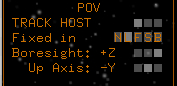
\includegraphics[width=2in]{POV.jpg} % requires the graphicx package
   \caption{The POV menu fixes the Point of View in a frame and aligns POV axes.}
   \label{fig:POV}
\end{figure}
The POV section selects the Point of View mode, fixes the POV in a reference frame, and aligns the POV axes.

The POV mode is TRACK HOST by default.  The other two choices (TRACK TARGET and FIXED IN HOST) aren't well developed.

The ``Fixed In'' selector aligns the POV axes with a particular reference frame, and places the POV's focus (center of attention) at a particular point.  The choices are:
\begin{itemize}
\item N:  The Inertial Frame.  The focus is the mass center of the spacecraft.
\item L:  The Local Vertical-Local Horizontal Frame.
\item F:  The Formation Frame.  The focus is the origin of the formation frame.
\item S:  The Spacecraft Frame.  The axes are aligned with the main body of the spacecraft.  The focus is the spacecraft mass center.
\item B:  The Body Frame.  The axes are aligned with those of the particular body selected in the Host section.  The focus is the origin of the selected body.
\end{itemize}

The Boresight selector aligns the boresight of the POV with a principal axis of the selected reference frame.  Clicking on a square selects the X, Y, or Z axis.  Clicking on the already-highlighted square changes the sign.

The Up Axis selector chooses which axis of the selected frame points up in the Cam window.  Note that the Up Axis can't be the same as the Boresight axis.  Changing the Boresight selection will also change the Up Axis to a default.  Adjust the Boresight first, then the Up Axis as desired.

The view may be rotated by clicking and dragging the mouse.  Known bug: clicking and dragging fails to rotate the view if the POV is fixed in L and the Host type is Body.

\section{The Host Section}

\begin{figure}[htb]
   \centering
   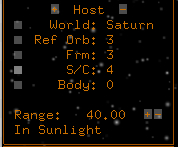
\includegraphics[width=2in]{Host.jpg} % requires the graphicx package
   \caption{The Host menu selects the POV's center of attention.}
   \label{fig:Host}
\end{figure}
The Host section selects the focus for the POV.  In most cases, the Host is a spacecraft, so the S/C button will be highlighted as shown.  Clicking on the ``+'' or ``-'' buttons on either side of the word Host will cycle through the active spacecraft.  The number next to S/C: identifies the current Host spacecraft.  Clicking the other radio buttons allows the user to focus the POV on some non-spacecraft options.  In particular, selecting Body allows focusing on a specific body of the selected spacecraft.

The Range may be increased or decreased by clicking the buttons in the Range line.  The number is the currect range in meters (or in radii, if the Host type is World).

The ``In Sunlight'' indicator simply calls out whether the host is in sunlight or in eclipse.

\end{document}


